\documentclass[11pt]{article}
\usepackage[top=2.54cm, left=2.54cm, right=2.54cm, bottom=2.54cm]{geometry}
\usepackage{amsmath}
\usepackage{float}
\usepackage{graphicx}
\usepackage{hyperref}
\usepackage{multicol}
\usepackage{multirow}
\hypersetup{colorlinks=true, urlcolor=blue,}
\usepackage{graphicx}

\begin{document}
% Title Page
\begin{titlepage}

	\centering
	{\Large Computational Physics \\ PHYS 3800 \par}
	\vspace{0.25cm}
	{\Large Final Project\par}
	\vspace{2cm}
	
	{\huge \textbf{ Rocket Propulsion} \par}
	\vspace{1cm}
	
	{\large Andrew Corp * \\ Department of Sciences, Wentworth Institute of Technology \\ 550 Hungtington Avenue, Boston, MA 02115}
	
		{\large Darrien Kennedy $\dagger$ \\ Department of Sciences, Wentworth Institute of Technology \\ 550 Hungtington Avenue, Boston, MA 02115}

	{\large \today \par}
\end{titlepage}
\newpage

{\centering \textbf{Abstract} \par}

Rocket Propulsion is a complicated physics topic that really came to be known in the late 60's and early 70's. Using the Saturn V's data, Euler's method, and the "Rocket Equation" we are able to calculate the velocity at any given time of a rocket through travel. We are also able to find connections between the payload and the thrust. 

\section{Introduction}
\par Saturn V was a rocket that started being constructed/researched in 1964, it was finished in 1967. This rocket was the largest and most powerful rocket built to date, it had 5 engines (which weighed 18,500 $lbs$ each). When the rocket was full with what it needed for the mission, it weighed about 6.5 million $lbs$. It was about 360 $ft$ tall, which is 60 feet taller than the Statue of Liberty! The rocket also generated about 7.6 million pounds of thrust at launch! 

\vspace{.25cm}
This rocket went on 13 missions, with only 1 partial failure. Most of these missions were the Apollo missions. The rocket had 3 stages, each used for a separate part of its trip to the moon. "The first stage lifted the rocket to an altitude of about 68 kilometers (42 miles). The second stage carried it from there almost into orbit. The third stage placed the Apollo spacecraft into Earth orbit and pushed it toward the moon. The first two stages fell into the ocean after separation. The third stage either stayed in space or hit the moon." \cite{saturnv}

\begin{figure}[H]
\centering
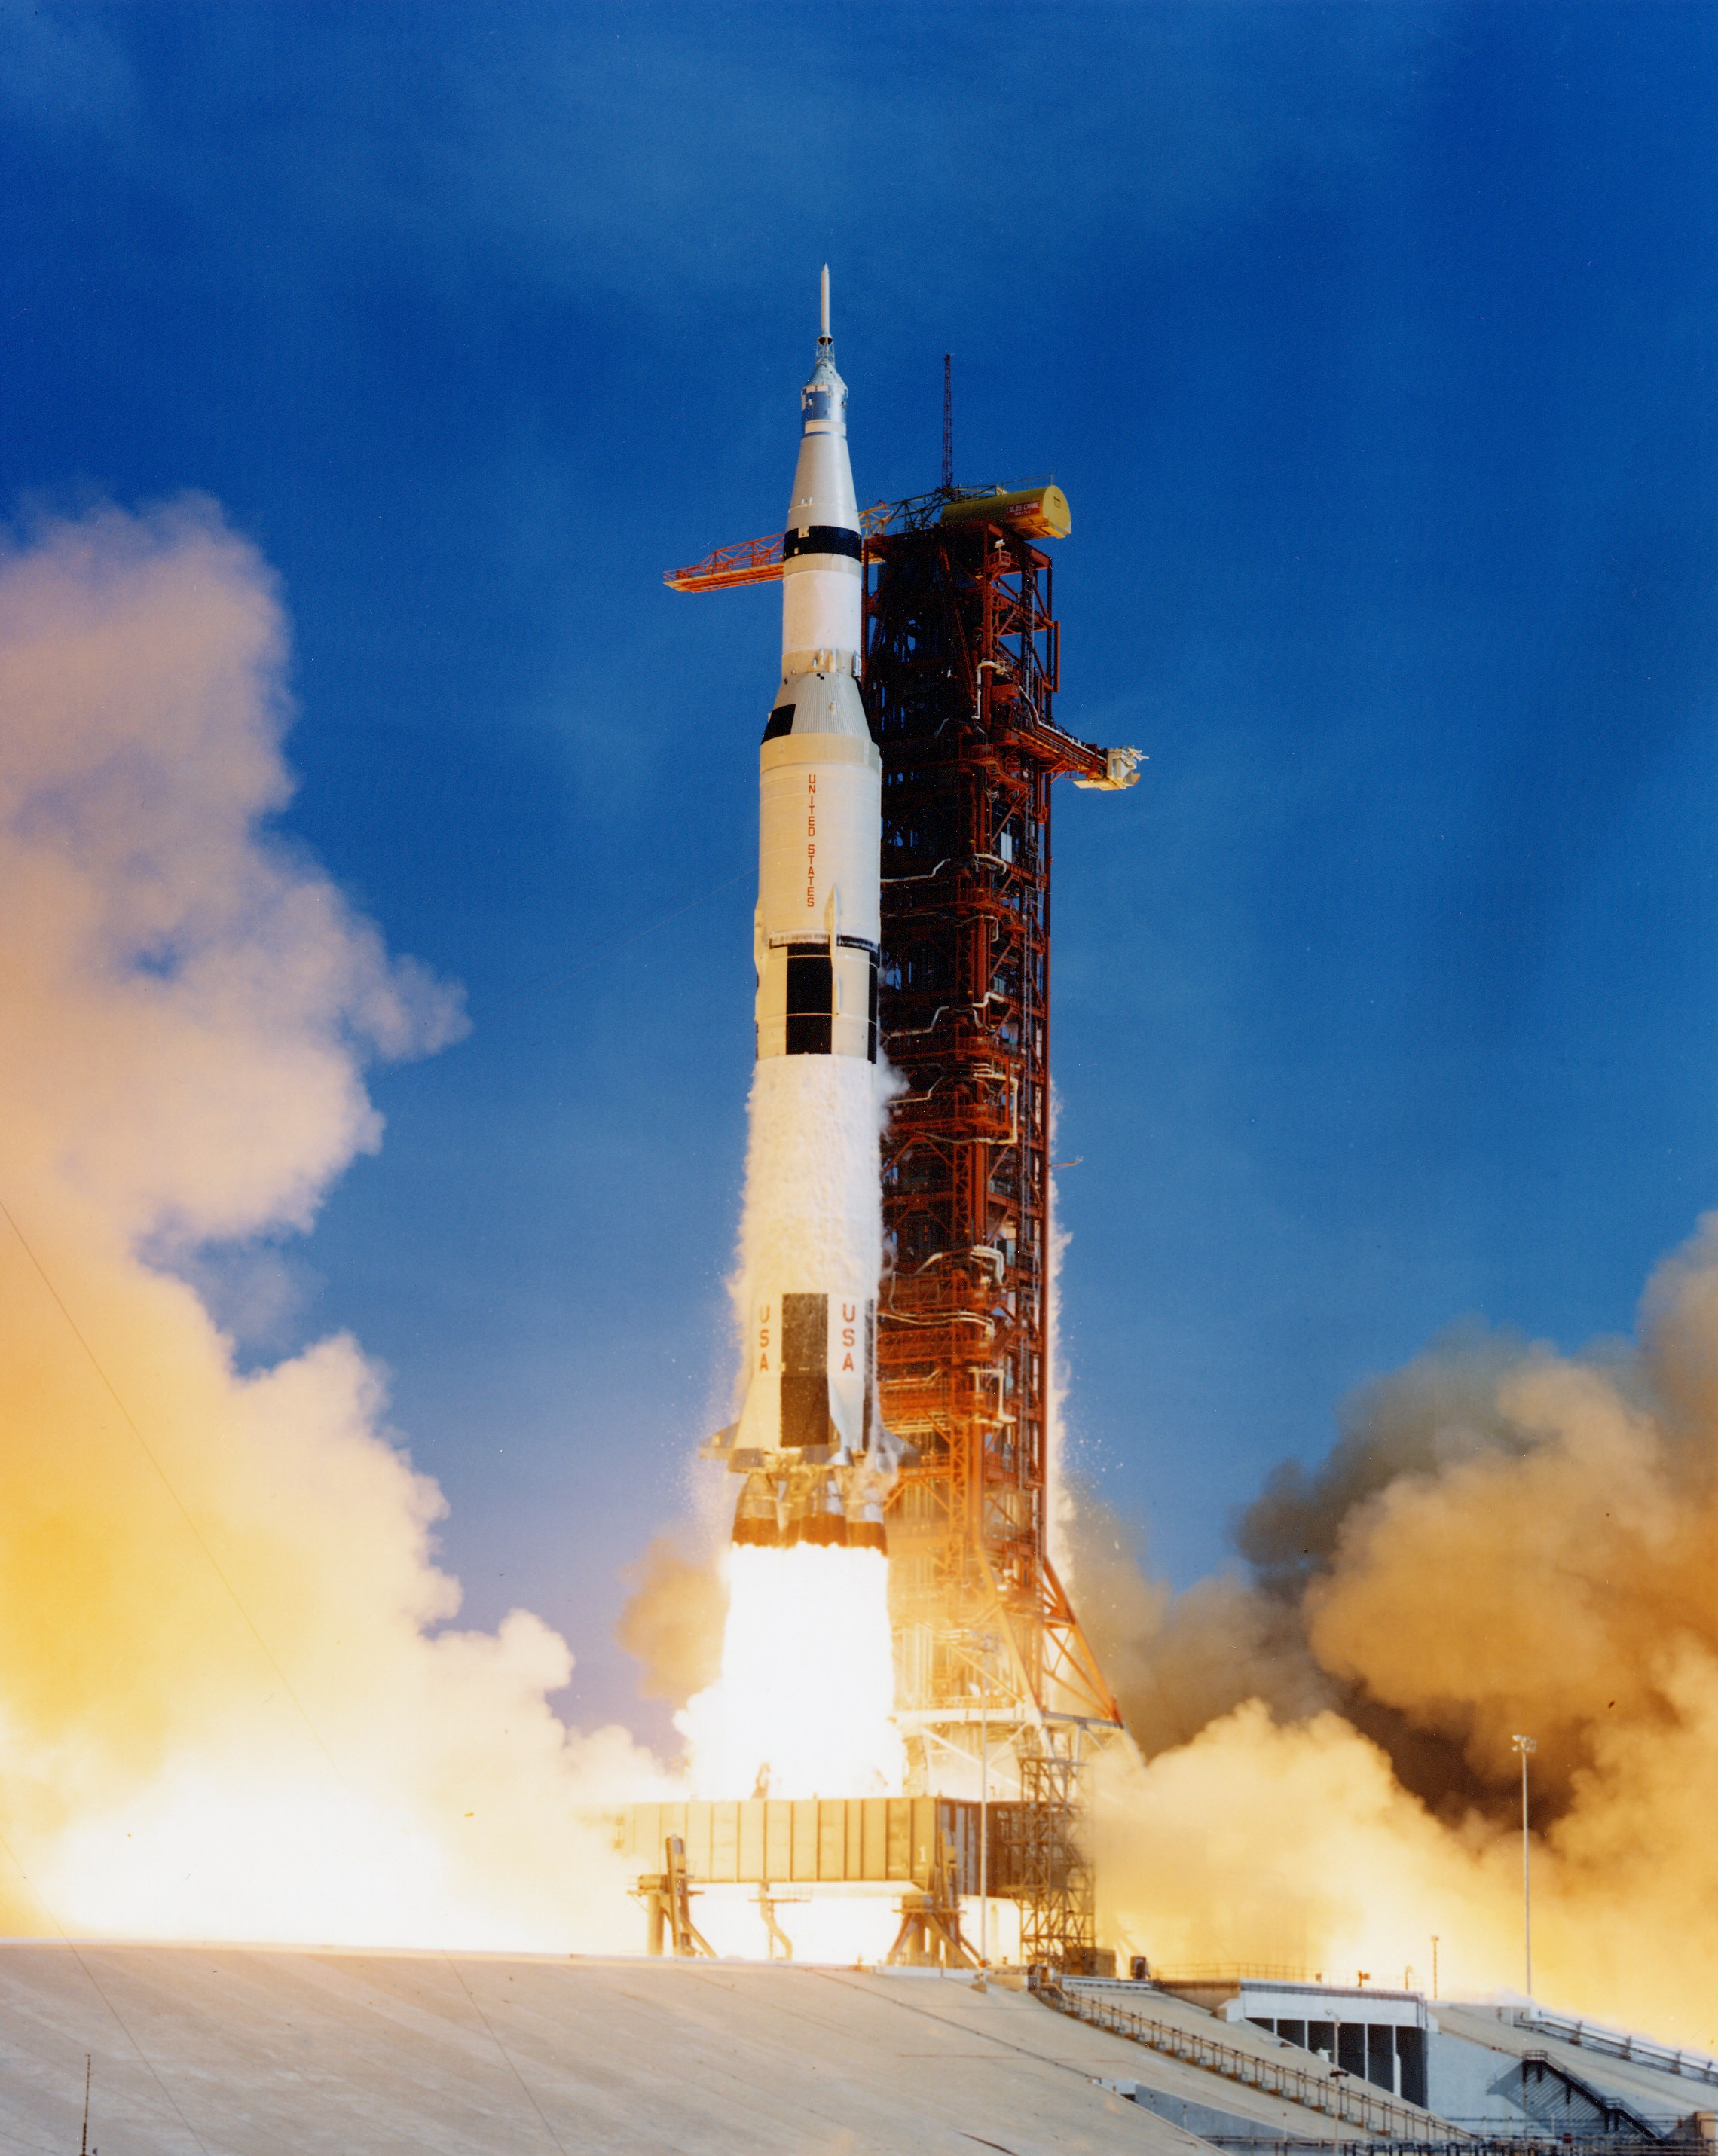
\includegraphics[scale=0.35]{SaturnV.jpg}
\caption{Saturn V - The most powerful and largest spaceship}
\end{figure}

\vspace{.25cm}

We decided to use Saturn V's rocket data, because of its remarkable accomplishments, for our calculations.

\section{Computational Method \& Techniques}
The rocket equation for a rocket's velocity can be derived from Newton's second law:
\begin{equation}
F = ma
\end{equation}
where $F$ is the force, $m$ is the mass of the object and $a$ is the acceleration. Knowing that the $Ru_{ex}$ also known as the force of thrust, is to be taken into account for the velocity of the rocket, which acceleration is the first derivative of velocity so the equation can be rewritten as

\begin{equation}
Ru_{ex} = m \frac{dv}{dt}
\end{equation}

\noindent and the equation for fuel mass would be 

\begin{equation}
m = m_i - Rt
\end{equation}

\noindent where $m_i$ is the initial mass, $R$ is the rate at which the fuel is burned (burn rate), and $t$ is the amount of time that has gone by. Incorporating this into our equation would result in

\begin{equation}
Ru_{ex} = (m_i - Rt) \frac{dv}{dt}
\end{equation}

\noindent and if we solve for $\frac{dv}{dt}$ it becomes

\begin{equation}
\frac{dv}{dt} = \frac{Ru_{ex}}{m_i - Rt}
\end{equation} 

Finally after accounting for the acceleration due to gravity from the rocket traveling out of our atmosphere we get our rocket equation

\begin{equation}\label{eq:rocketeq}
\frac{dv}{dt} = \frac{Ru_{ex}}{m_i-Rt}-g
\end{equation}

Of course it should be noted that with the rocket equation we are not accounting for air resistance. As you likely know, air resistance is the force acting against the rocket as it exits the atmosphere, which would mean that the results from our calculations should not be taken literally.

\begin{equation}
\int{dv} = \int{\frac{Ru_{ex}}{m_i-Rt}} - \int{g dt}
\end{equation}

\begin{equation}
v_f-v_o = Ru_{ex}\int{\frac{1}{m_i-Rt}}dt - gt
\end{equation}

pull out the mass

\begin{equation}
v = Ru_{ex}\int{\frac{1}{1-\frac{Rt}{m_i}}}dt - gt
\end{equation}
Apply Integral substitution denoted with $p$, where
$p = 1-\frac{Rt}{m_i}$, and
$dp = - \frac{R}{m_i}dt$

\begin{equation}
\int{\frac{1}{u}(-\frac{m_i}{R})du}
\end{equation}
\begin{equation}
- \frac{m_i}{uR}
\end{equation}
\begin{equation}
\int{-\frac{m_i}{Ru} du}
\end{equation}

Take the constant out
\begin{equation}
-\frac{m_i}{R} \int{\frac{1}{u}du}
\end{equation}

\begin{equation}
= -\frac{m_i}{R}ln|u|
\end{equation}

\begin{equation}
= -\frac{m_i}{R}ln|\frac{1}{1-\frac{Rt}{m_i}}|
\end{equation}

The approximation is calculated using Euler's method which is pretty easy to grasp as

\begin{equation}
next = previous + dt * f(x)
\end{equation}

\noindent where our function is $\frac{dv}{dt}$ instead of $f(x)$. The value for the approximate velocity is initialized to zero and gradually builds up over time.


\section{Implementation}
For implementation, we wrote a FORTRAN 90 program which calculates the exact values and approximate values of the time until the rocket burns all of its fuel. The percent error is also calculated from the difference between the exact value and approximate value. Finally the mass of the fuel is calculated over time. All four of these calculation's values are stored in respective files in order to allow for easy plotting of the data using \textit{Xmgrace}. The data files are \textbf{rocket.dat} for the approximate value, \textbf{rocket\_exact.dat} for the exact value, \textbf{error.dat} for the percent error, and \textbf{mass\_change.dat} for the change in fuel mass over time.\\

The user is prompted for a timestep which they would like to be used for the program, the lower timestep the more data is generated and the more precise the graphs will appear. We then use the initial values based off of the Saturn-V rocket specifications and calculate the time at which all of the fuel is exausted. Then in a while loop we loop through while a time value, which is initialized to zero, is less than the calculated burn time. In this loop is where all of our calculations are performed, in calculating the exact value, approximate value, percent error and fuel mass. The files are then updated with their respective values in relation to time. Finally the time is then updated based off of the timestep. After the loop is complete, the files are closed and the program terminates.

\section{Results}
As said above, we used \textit{Xmgrace} to create graphs of the data that was outputted from the calculations with FORTRAN. We decided to create four graphs:
%two of which are for the velocities at different time steps one is for the percent error generated  and the other 

\vspace{0.25cm}

\newpage
This graph shows how well Euler's method does to approximate the rocket calculation. It is impossible to tell that there is a difference in the approximation and the exact velocity while the time step is .01 seconds. As the legend shows, the black circles (and line) is the approximation while the red line is the exact.
\begin{figure}[H]
\centering
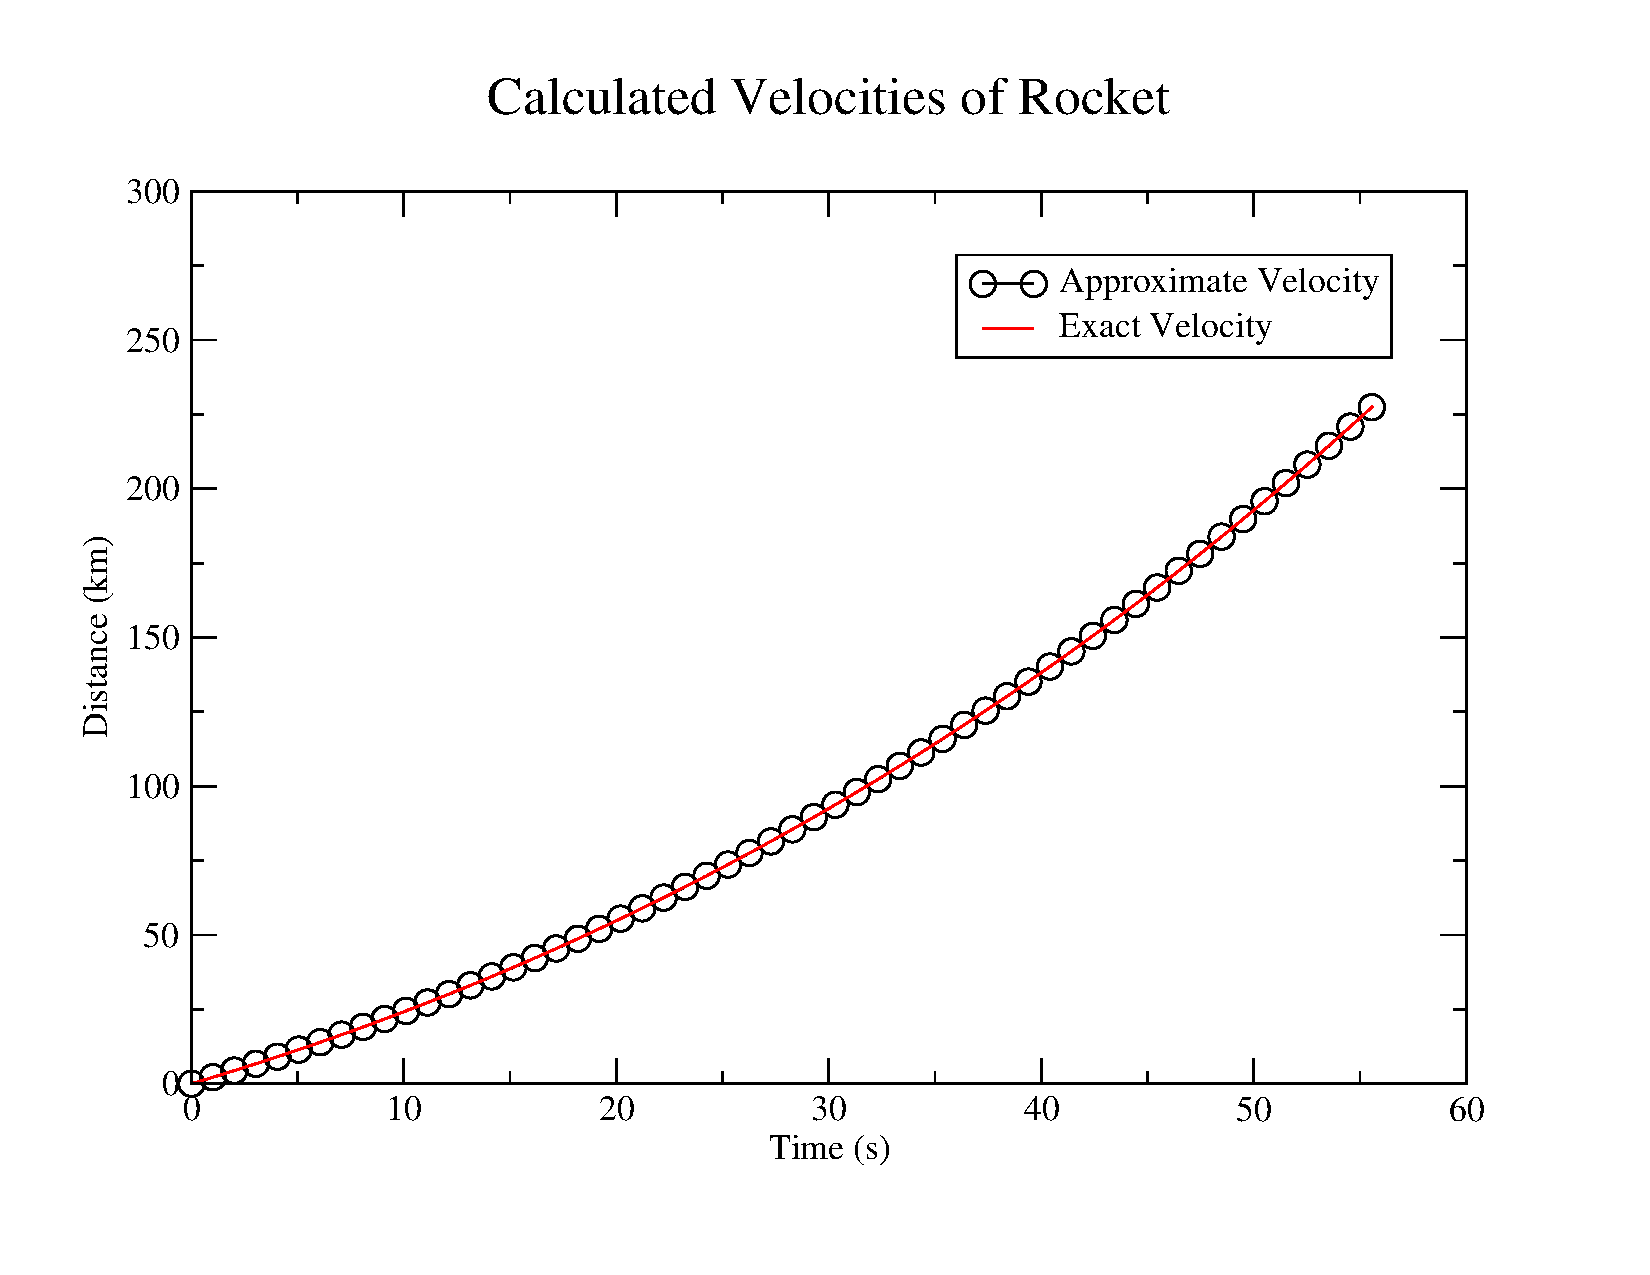
\includegraphics[scale=0.45]{velocity01.pdf}
\caption{Velocities when dt = 0.01}
\end{figure}
\newpage
Looking at this graph you can see that the two lines arent the same. This shows how when you change the time step to be at 2 seconds, Euler's method looks to be not as good. This makes sense because in this case Euler's method is not being iterated as many times, therefore not generating as many datapoints and skipping over some points of the line.
\begin{figure}[H]
\centering
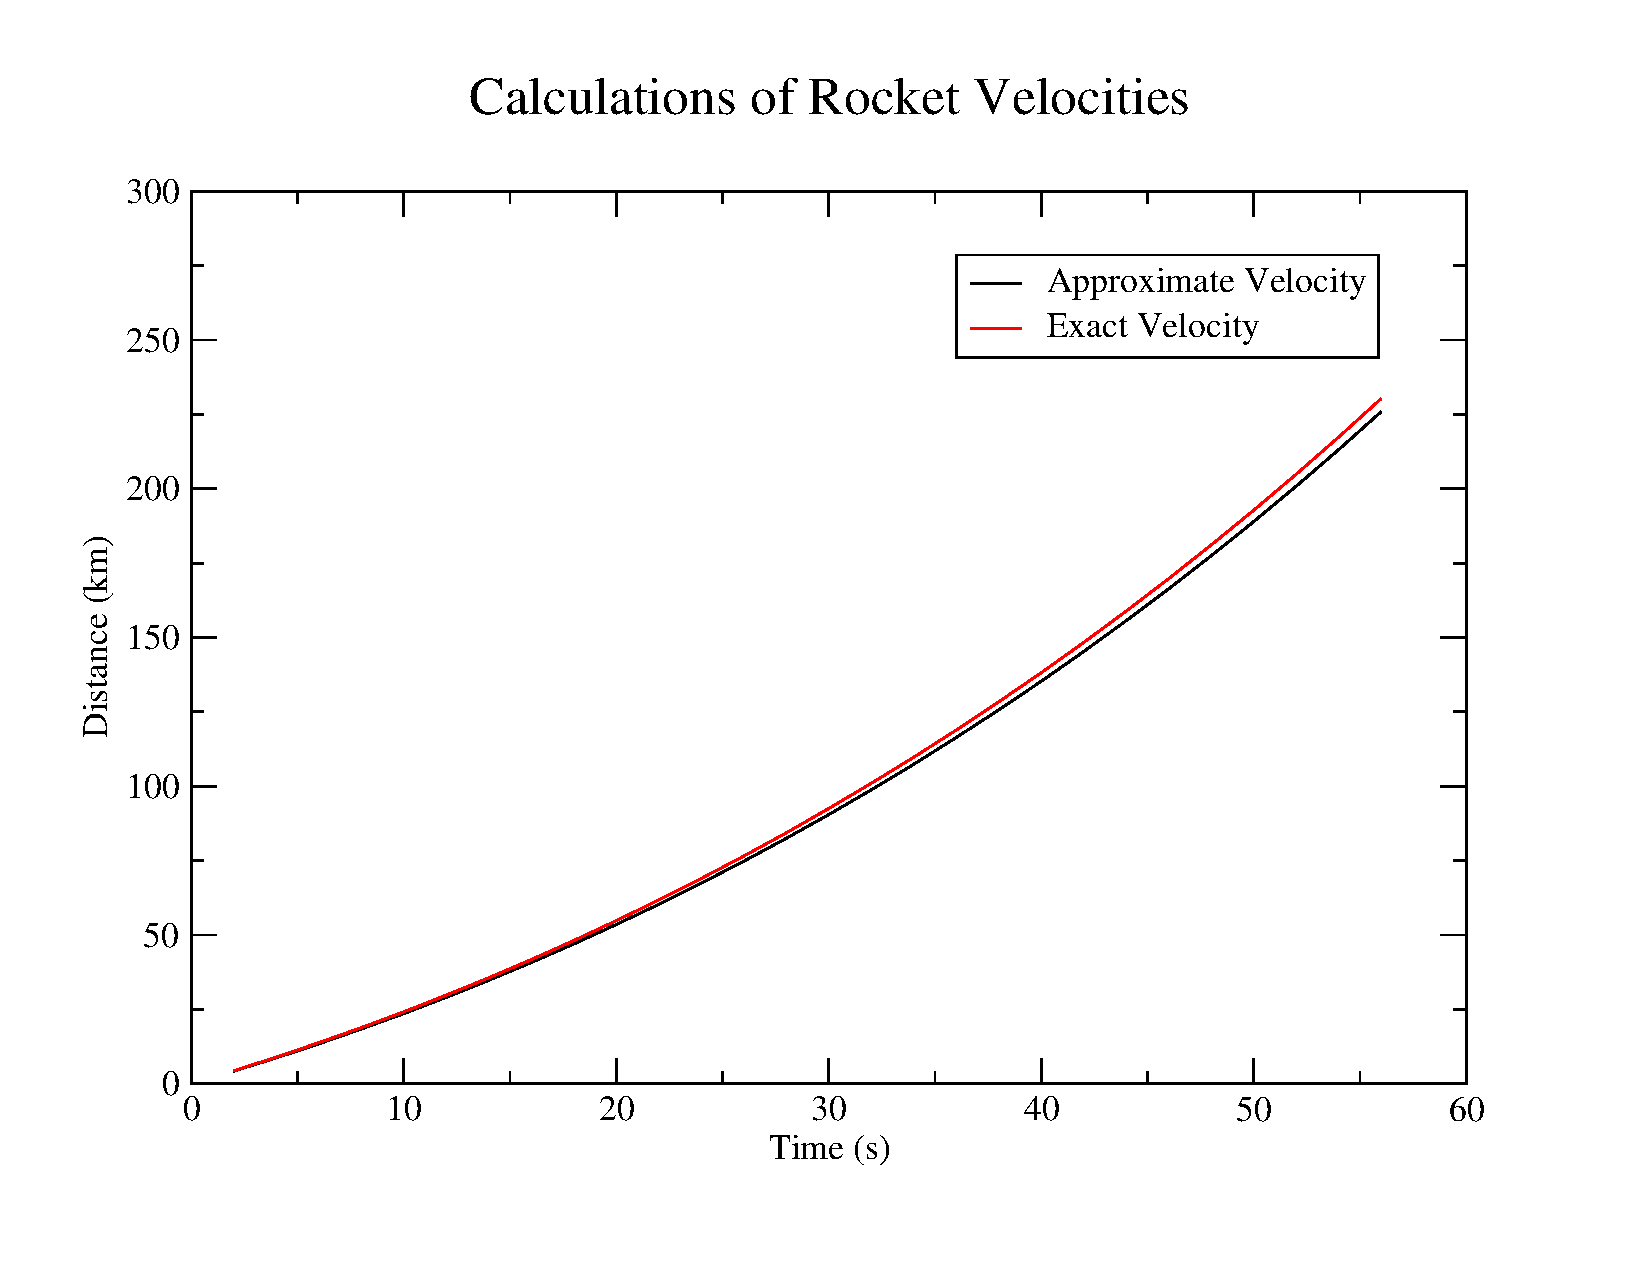
\includegraphics[scale=0.45]{velocity2.pdf}
\caption{Velocities when dt = 2}
\end{figure}
\newpage
Here is the percent error between the approximate and the exact:
\begin{figure}[H]
\centering
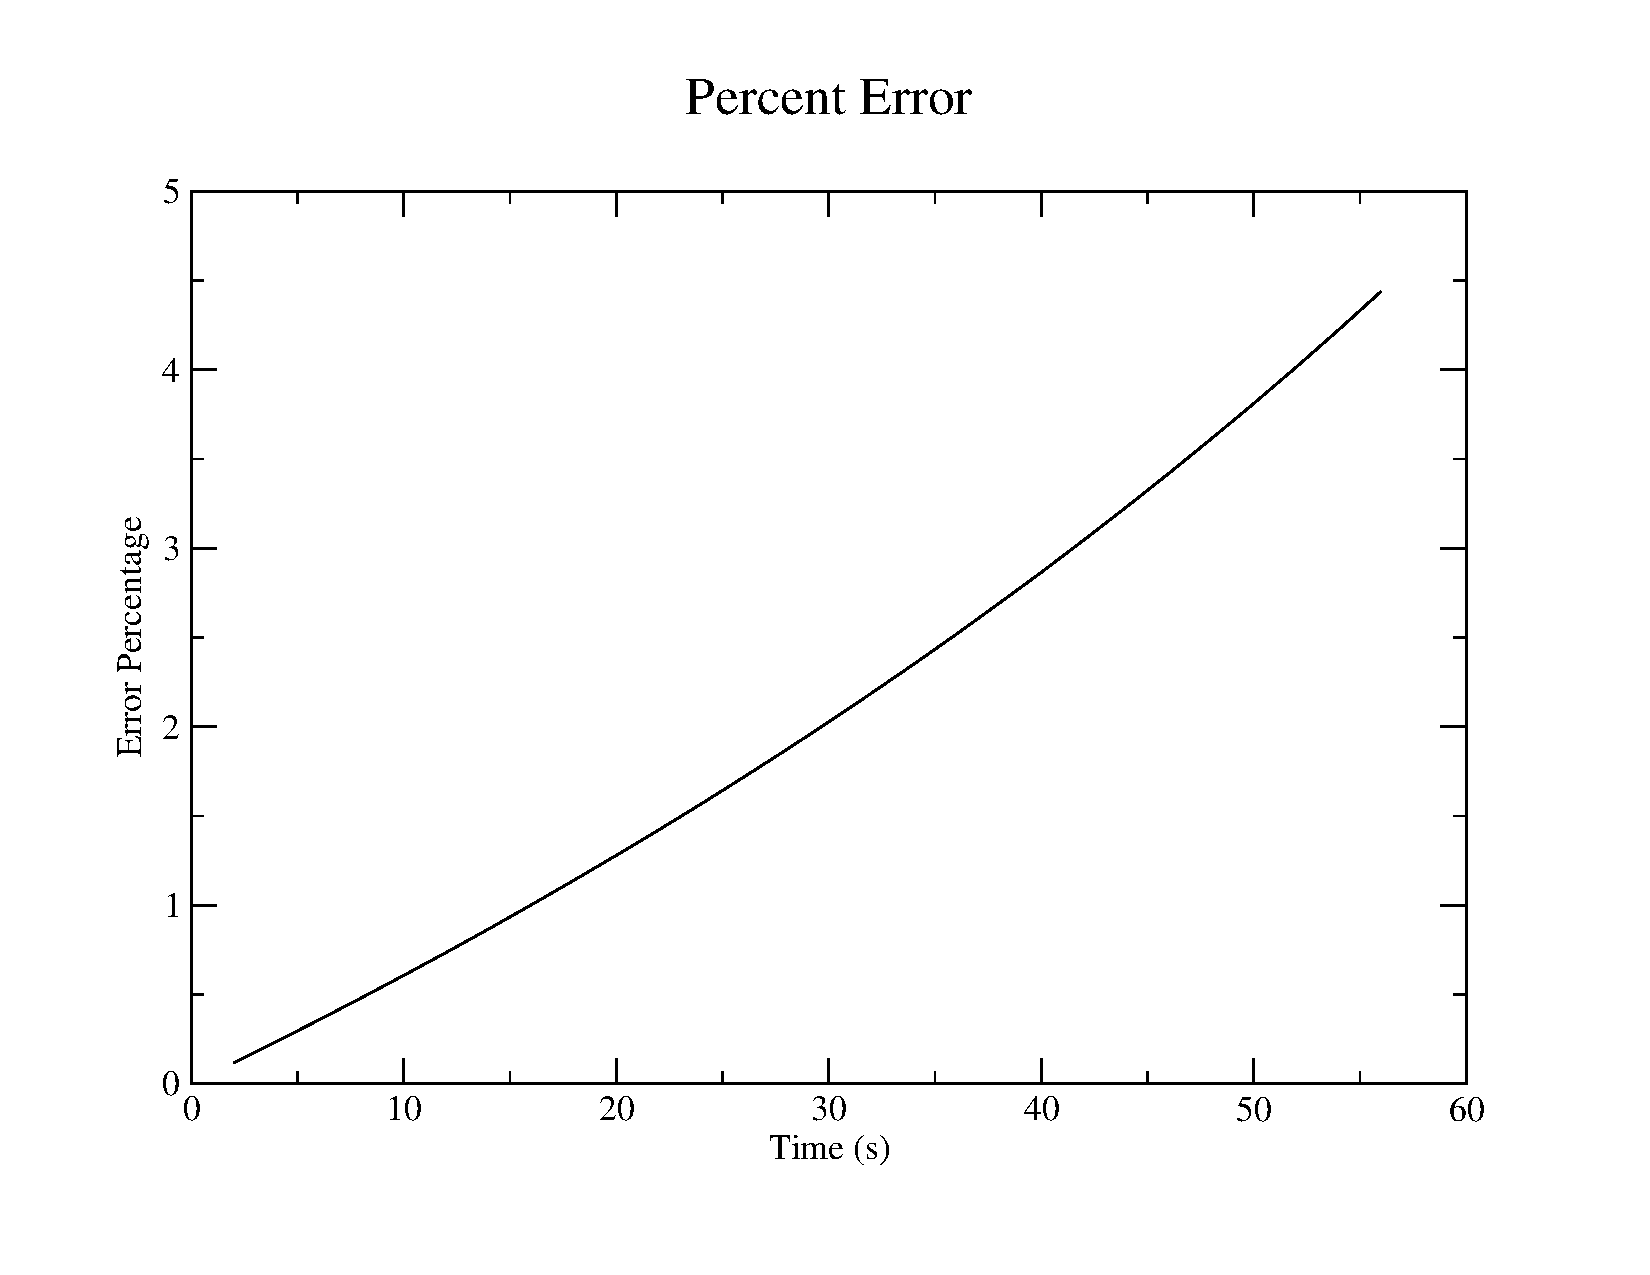
\includegraphics[scale=0.45]{error.pdf}
\caption{Percent Error when dt = 2}
\end{figure}
\newpage
Lastly, here is the graph of the change of mass over time. This is linear because looking at equation \eqref{eq:rocketeq} you can see that the denominator is $m_i - Rt$, which is linear, and this is what determines the current fuel at a given time. Also, the fuel mass does reach zero (after it burns all of the fuel).

\begin{figure}[H]
\centering
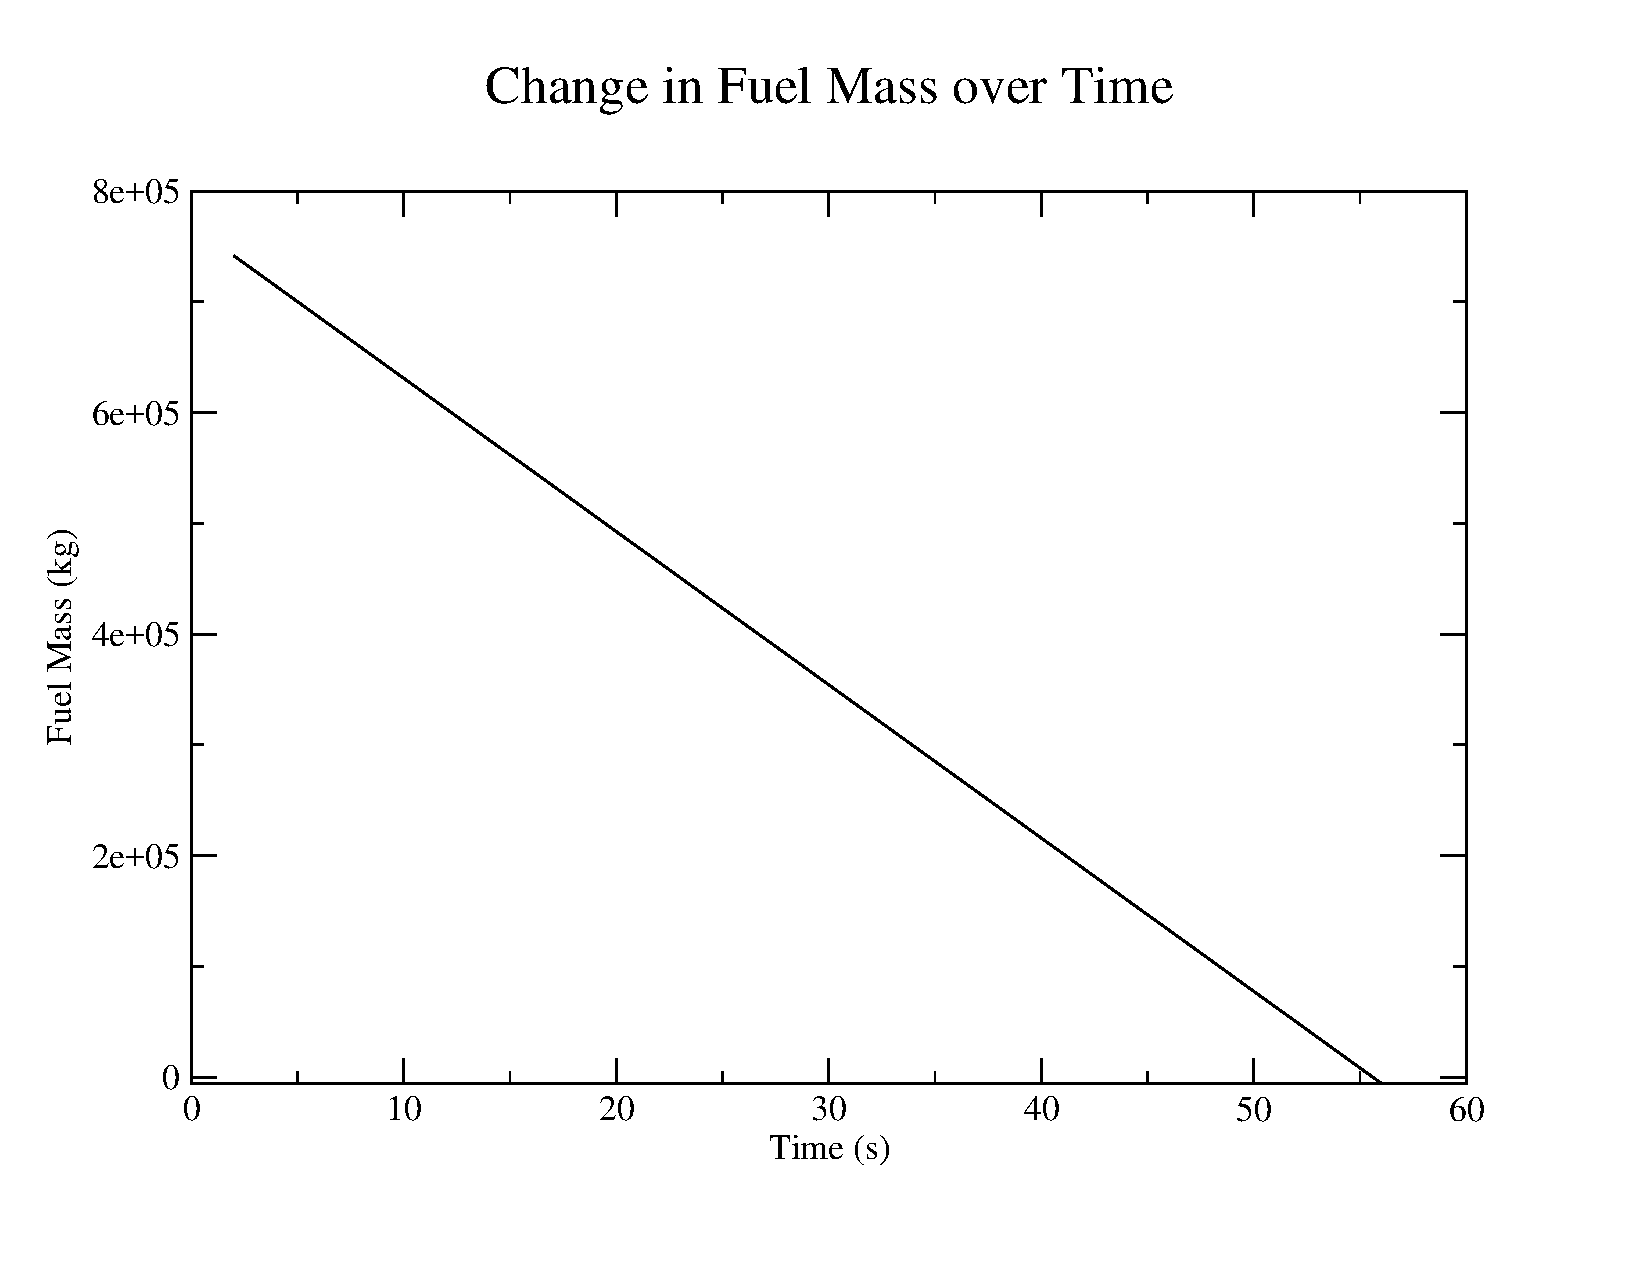
\includegraphics[scale=0.45]{fuelMassChange.pdf}
\caption{Fuel Change over Time}
\end{figure}

\section{Conclusion}
As you can see, by looking at the plots you can tell a few things. One of which is Euler's method does a great job when you perform many iterations, but not as well when you don't. Looking at the first plot compared to the second, Euler's doesn't do great and that is because of this. To prove that error exists when the time step is 2 seconds, there is a graph to show it. It nearly gets to 5 \% error. I believe that even though we decided not to account for air resistance, the code that we have written will be able to calculate the correct exact equation and use Euler's method correctly. By using these 2 equations we are able to see how a rocket speeds up over time and we are able to see the connection between payload and thrust.

\newpage
\begin{thebibliography}{9}

	\bibitem{spaceflight}
		\textit{Basics of Space Flight - Rocket Propulsion}, \textcolor{blue}{http://www.braeunig.us/space/propuls.html}
	\bibitem{nasa}
		\textit{NASA - Rocket Propulsion}, \textcolor{blue}{https://www.grc.nasa.gov/www/K-12/airplane/rocket.html}
	\bibitem{saturnv}
   	 	\textit{What Was the Saturn V?}, \textcolor{blue}{https://www.nasa.gov/audience/forstudents/5-8/features/nasa-knows/what-was-the-saturn-v-58.html}

\end{thebibliography}

\end{document}